% !TEX root = ../main.tex
\section{Absorption Coefficient and Gain}
\label{sec:absorption_coefficient_and_gain}

The absorption coefficient $\alpha(\hbar \omega)$ is a fundamental material property,
used in the Lambert-Beer law $I(z)=I_{0}\exp(-\alpha z)$, which describes the decay
of the light intensity $I$ with the propagation distance $z$. The absorption
coefficient can be defined universally as:
\begin{equation}
	\alpha =\frac{\text{Number of photons absorbed per second per unit volume}}{\text{Number
	of injected photons per second per unit area}}.\label{eq:alpha}
\end{equation}
The numerator of \cref{eq:alpha} is the net absorption rate,
$R^{\mathrm{abs}}- R^{\mathrm{stim}}$ emission. Using its analytical form from \cref{sec:line_shape}
results in:
\begin{equation}
	R^{\mathrm{net}}=n_{\mathrm{ph}}(r^{\mathrm{abs}}-r^{\mathrm{stim}}) = n_{\mathrm{ph}}
	\, P(\hbar\omega) \lvert \hat{e}\cdot \mathbf{p}_{\mathrm{cv}}\rvert^{2}D_{\mathrm{j}}
	(\hbar\omega)\,(1-f_{\mathrm{n}}-f_{\mathrm{p}}).
\end{equation}
The denominator is the spectral photon flux, i.e. the number of injected photons
crossing a unit area per second per photon energy. This quantity is obtained from
the spectral photon density $S=n_{\mathrm{ph}}N$, travelling at the velocity
$c/n_{\mathrm{r}}$:
\begin{equation}
	F=n_{\mathrm{ph}}\cdot N \cdot \frac{c}{n_{\mathrm{r}}}= n_{\mathrm{ph}}\frac{n_{\mathrm{r}}^{2}\omega^{2}}{\pi^{2}\hbar
	c^{2}}.
\end{equation}

Dividing $R_{\mathrm{net}}$ by $F$ cancels $n_{\mathrm{ph}}$ and yields an
analytical expression for the absorption coefficient:
\begin{equation}
	\alpha(\hbar \omega)=\frac{R^{\mathrm{net}}}{F}=C_{0}\lvert \hat{e}\cdot\mathbf{p}
	_{\mathrm{cv}}\rvert^{2}D_{\mathrm{j}}(1-f_{\mathrm{n}}-f_{\mathrm{p}}). \label{eq:alpha_analytical}
\end{equation}

\subsection{Thermal Equilibrium}

In an undoped, unexcited semiconductor at low temperature ($k_{\mathrm{B}}T\ll E_{\mathrm{g}}$),
the valence band is full and the conduction band is empty,
$f_{\mathrm{n}}\approx 0$ and $f_{\mathrm{p}}\approx0$. The expression above then
reduces to the equilibrium absorption coefficient $\alpha_{0}$. The
approximation is valid if the considered energy interval is small:
\begin{equation}
	\alpha_{0}(\hbar \omega)=C_{0}\lvert \hat{e}\cdot \mathbf{p}_{\mathrm{cv}}\rvert
	^{2}D_{\mathrm{j}}\propto \frac{\sqrt{ \hbar \omega -E_{\mathrm{g}}}}{\hbar
	\omega}\simeq \sqrt{ \hbar \omega -E_{\mathrm{g}}}.
\end{equation}

\subsection{Non-Equilibrium and Bernard-Duraffourg Condition}

Away from equilibrium, $f_{\mathrm{n}}$ and $f_{\mathrm{p}}$ are governed by
separate quasi-Fermi levels, so $1-f_{\mathrm{n}}-f_{\mathrm{p}}$ can in principle
change sign. To this end, the occupation factor in \cref{eq:alpha_analytical} is rewritten
using \cref{eq:f_n_identity} with $E_{\mathrm{c}}(k_{0})-E_{\mathrm{v}}(k_{0})=\hbar
\omega$:
\begin{align}
	1-f_{\mathrm{n}}-f_{\mathrm{p}} & =(1-f_{\mathrm{n}})(1-f_{\mathrm{p}}) - f_{\mathrm{n}}f_{\mathrm{p}}=f_{\mathrm{n}}f_{\mathrm{p}}\left[ \frac{(1-f_{\mathrm{n}})(1-f_{\mathrm{p}})}{f_{\mathrm{n}}f_{\mathrm{p}}}- 1\right] \\
	                                & =f_{\mathrm{n}}f_{\mathrm{p}}\left[\exp\left( \frac{\hbar \omega -(F_{\mathrm{n}}-F_{\mathrm{p}})}{k_{\mathrm{B}}T}\right) -1\right]. \label{eq:f_n_identity_2}
\end{align}

Substituting \cref{eq:f_n_identity_2} into $\alpha(\hbar\omega)$ with the parabolic-band
joint density of states gives, with all energy-independent prefactors collected
in a constant:
\begin{equation}
	\alpha(\hbar \omega) = \underbrace{ \mathrm{const.} }_{ >0 }\; \underbrace{ \frac{\sqrt{
	\hbar \omega-E_{\mathrm{g}}}}{\hbar \omega} }_{ \hbar \omega >E_{\mathrm{g}} }\;
	\underbrace{ f_{\mathrm{n}} }_{ >0 }\; \underbrace{ f_{\mathrm{p}} }_{ >0 }\; \underbrace{
	\left[\exp\left( \frac{\hbar \omega -(F_{\mathrm{n}}-F_{\mathrm{p}})}{k_{\mathrm{B}}T}
	\right) -1\right] }_{ <0 \text{ if } \hbar \omega <F_{\mathrm{n}}-F_{\mathrm{p}}
	}.
\end{equation}
Only the bracket can change sign; every other factor in the expression is
positive. A negative value of the bracket corresponds to gain instead of absorption.
The bracket is negative exactly when
$\hbar\omega < F_{\mathrm{n}}-F_{\mathrm{p}}$; combined with the requirement $\hbar
\omega>E_{\mathrm{g}}$ for the transition to exist at all, this gives the
Bernard-Duraffourg condition: $F_{\mathrm{n}}-F_{\mathrm{p}}>\hbar \omega > E_{\mathrm{g}}$.

\subsection{Gain}

The gain $g$ is the key quantity of an active medium: the intensity of light passing
through it grows exponentially instead of decaying:
\begin{equation}
	I(z)=I_{0}\, \exp(g z).
\end{equation}

% \begin{table}[H]
% \centering
% \begin{tabular}{p{0.32\textwidth}p{0.32\textwidth}p{0.32\textwidth}}
% \toprule
% Symbol & Meaning & Unit \\
% \midrule
% $I(z), I_0$ & light intensity at position $z$ / at $z=0$ & $\mathrm{W\,m^{-2}}$ \\
% $z$ & propagation distance in the medium & $\mathrm{m}$ \\
% $g$ & material gain coefficient & $\mathrm{m^{-1}}$ \\
% \bottomrule
% \end{tabular}
% \caption{TODO}
% \end{table}

The gain coefficient is the negative of the absorption coefficient, so Lambert-Beer
absorption turns into amplification:
\begin{equation}
	g(\hbar\omega)=-\alpha(\hbar\omega)=C_{0}\lvert \hat{e}\cdot\mathbf{p}_{\mathrm{cv}}
	\rvert^{2}D_{\mathrm{j}}\,(f_{\mathrm{n}}+f_{\mathrm{p}}-1).
\end{equation}

% \begin{table}[H]
% \centering
% \begin{tabular}{p{0.32\textwidth}p{0.32\textwidth}p{0.32\textwidth}}
% \toprule
% Symbol & Meaning & Unit \\
% \midrule
% $g$ & material gain coefficient & $\mathrm{m^{-1}}$ \\
% $\alpha$ & macroscopic absorption coefficient & $\mathrm{m^{-1}}$ \\
% $\hbar\omega$ & photon energy & $\mathrm{J}$ (often eV) \\
% $C_0$ & coupling prefactor of the electron-light interaction & $\mathrm{m^{2}\,kg^{-1}}$ \\
% $\hat{e}$ & unit polarization vector of the light field & dimensionless \\
% $\mathbf{p}_{\mathrm{cv}}$ & momentum matrix element between conduction- and valence-band Bloch states & $\mathrm{kg\,m\,s^{-1}}$ \\
% $D_{\mathrm{j}}$ & joint density of states, see Joint Density of States & $\mathrm{m^{-3}\,J^{-1}}$ \\
% $f_{\mathrm{n}}, f_{\mathrm{p}}$ & probability that a conduction-band state is occupied by an electron / a valence-band state by a hole & dimensionless \\
% \bottomrule
% \end{tabular}
% \caption{TODO}
% \end{table}

The gain curve $g(\hbar\omega)$ follows from the sign analysis above and is
depicted in \cref{fig:absorption_gain}: $g=0$ below $E_{\mathrm{g}}$, since no
transitions exist there; $g>0$ between $E_{\mathrm{g}}$ and $F_{\mathrm{n}}-F_{\mathrm{p}}$,
rising with the joint density of states and falling with
$f_{\mathrm{n}}+f_{\mathrm{p}}-1$. $g=0$ at the transparency energy $\hbar\omega=
F_{\mathrm{n}}- F_{\mathrm{p}}$ and $g<0$ above it, approaching the equilibrium
absorption $-\alpha_{0}$ at high photon energies.

\begin{figure}[H]
	\centering
	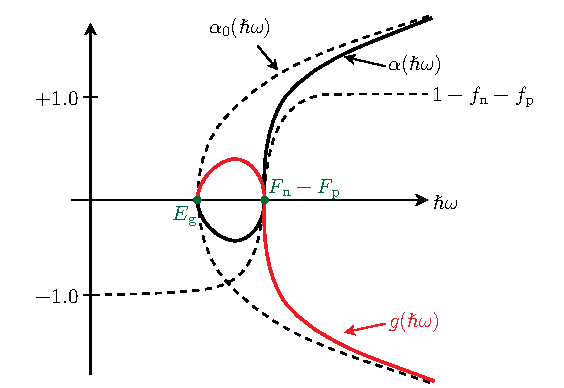
\includegraphics[width=0.6\linewidth]{../assets/absorption_gain.pdf}
	\caption{Absorption coefficient $\alpha(\hbar\omega)$ under carrier injection
	(solid) compared to the equilibrium absorption $\alpha_{0}(\hbar\omega)$ (dashed).
	The factor $1-f_{\mathrm{n}}-f_{\mathrm{p}}$ (dashed) changes sign at $\hbar\omega
	=F_{\mathrm{n}}-F_{\mathrm{p}}$. The gain
	$g(\hbar\omega)=-\alpha(\hbar\omega)$ is shown in red. \imcite{chuang_physics_2009}}
	\label{fig:absorption_gain}
\end{figure}

Note that $g$ is the material gain of the active medium alone. The gain
experienced by a guided optical mode is reduced to the modal gain $\Gamma g$ by
the optical confinement factor $\Gamma$. Lasing additionally requires this modal gain
to overcome the internal losses and the mirror losses (see
\cref{sec:resonator_and_threshold}).

% Gliederung: Brücke zu Kapitel 4: der Fabry-Perot-Resonator braucht $g$ für die Schwellbedingung $\Gamma g_{\mathrm{th}}=\alpha_{\mathrm i}+\alpha_{\mathrm m}$